% !TEX root = % !TEX root = /Users/nai1ka/Projects/PerfX/Thesis/thesis.tex

\chapter{Methodology}
\label{chap:met}

This chapter describes the design of the proposed performance monitoring system. Section~\ref{sec:req} lists the requirements that influenced the design choices. Section~\ref{sec:arch} gives a high-level overview of the architecture and shows how the components work together. Sections~\ref{sec:sdk},~\ref{sec:backend} describe the details of the mobile SDK and the backend server. Section~\ref{sec:detection} discusses the regression detection methods that were considered and highlights the selected one.

\section{System requirements and constraints}
\label{sec:req}

Since the SDK (Software Development Kit) runs on real user devices, it must be lightweight so that it doesnt affect the user experience of the host application. Moreover, the system must be robust across different Android devices. Finally, regression detection must be reliable and resilient to outliers, as production data is often noisy.

\section{High-Level System Architecture}
\label{sec:arch}

The system consists of four components: the mobile SDK (client), the backend server, the frontend, and the regression detection engine. Figure~\ref{fig:system_architecture} shows how they are connected.

The mobile SDK is a library that developers integrate into their Android applications. It collects performance metrics on users' devices and sends them to the backend for further analysis.

The backend receives metrics from user devices, stores them efficiently, and provides REST APIs for the frontend. It is also responsible for user authentication and project management.

The frontend is a web application that lets developers manage projects, browse metrics, configure alerts, and review detected regressions. It interacts with the backend through REST APIs to retrieve data and present it in a user-friendly way.

The regression detection engine continuously analyses the incoming metrics to find signs of performance degradation. If such a regression is detected, it sends an alert to developers using the configured notification channels.

% \begin{figure}[htbp]
%     \centering
%     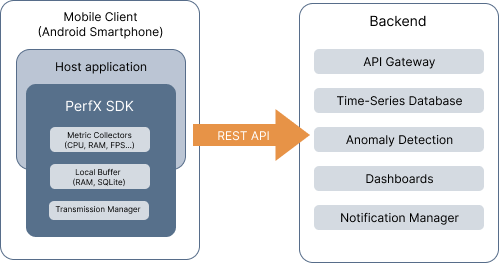
\includegraphics[width=0.8\textwidth]{figs/system_architecture.png}
%     \caption{High-Level System Architecture}
%     \label{fig:system_architecture}
% \end{figure}

\begin{figure}[htbp]
    \centering
    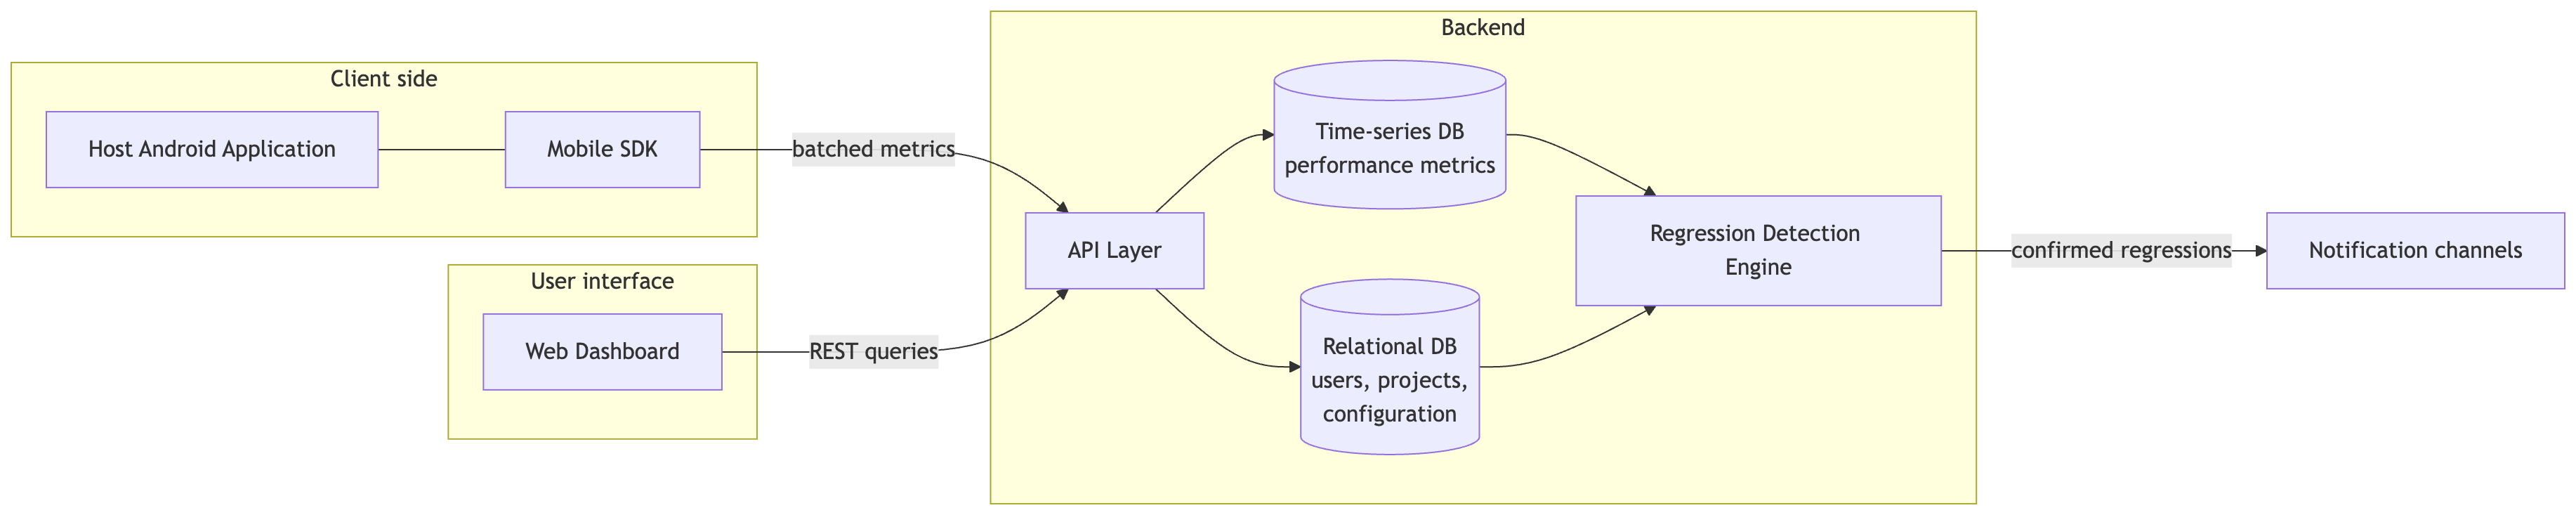
\includegraphics[width=1\textwidth]{figs/system_architecture_new.png}
    \caption{High-Level System Architecture}
    \label{fig:system_architecture}
\end{figure}

\section{Mobile SDK Design}
\label{sec:sdk}

\subsection{Metrics Selection and Collection}

Metrics selection was based on the literature review. They are divided into two major categories: continuous metrics and discrete events. Continuous metrics, such as CPU usage and frame time, are sampled at regular intervals. Discrete events, such as crashes, ANRs, and app startups, are recorded immediately when they happen. This approach allows the system to capture both the ongoing performance of the application and the rare but critical events that can significantly affect user experience.

\subsection{UI performance metrics}

For UI performance, the SDK tracks frame time, FPS, startup time, interaction delays, and ANR events.

\textbf{Frame time} is one of the most important metrics for measuring UI responsiveness. It represents the time needed to render a single frame of the user interface. The target frame time depends on the display refresh rate of the device. For example, on a 60 Hz display, the frame time should stay below approximately 16.67 ms in order to keep animations and interactions smooth \cite{android_slow_rendering}.

Frame time is measured by recording the timestamps of two consecutive frames and calculating the difference between them. If $t_i$ and $t_{i-1}$ are the timestamps of two consecutive frames, the frame time is calculated as follows:
\begin{equation}
    FrameTime(ms) = \frac{t_i - t_{i-1}}{10^6}
\end{equation}

\textbf{Frames per second (FPS)} is a related metric that is derived directly from the frame time. It is calculated as:
\begin{equation}
    FPS = \frac{1000}{FrameTime(ms)}
\end{equation}

\textbf{User interaction delay} measures the time between a user action (e.g. tap on a screen or a swipe) and the first visible response of the application. It is obtained by recording the timestamp of the user event and the timestamp of the first frame that was rendered after the event was processed. The delay is then calculated as:
\begin{equation}
    InteractionDelay(ms) = t_{\text{response}} - t_{\text{event}}
\end{equation}

\textbf{Startup time} shows how long the application takes to become visually responsive after it has been launched. It is defined as the time difference between the moment the application starts and the moment when the first fully rendered frame is drawn on the screen.

\textbf{ANR (Application Not Responding) events} happen when the application is unable to handle user input for a long period of time. This is a critical metric, because ANRs directly affect user experience and can lead to the application being terminated by the operating system. ANR events are detected by monitoring the main thread. If the main thread remains blocked for more than a predefined threshold (for example, 5 seconds), an ANR event is recorded.

\subsection{CPU usage}

There are several ways to measure CPU usage on Android. The method selected in this work is based on the ratio between the CPU time used by the application process and the total CPU time of the system during the same interval. The main advantage of this approach is that it does not depend on the number of CPU cores or on their frequencies, which gives a normalized measure of CPU usage. This property is important, because the collected values can be compared across different devices in a fair way. On the other hand, this method may miss short-term spikes that happen between two sampling intervals. However, this is not a problem in the context of this work, because the main goal is to detect long-term performance degradation rather than short spikes of load. It is calculated as follows:

Let $\Delta P$ be the increase in process CPU time and $\Delta S$ be the increase in total system CPU time during the same period. Then the CPU usage of the application is calculated as:
\begin{equation}
    CPU\% = \frac{\Delta P}{\Delta S} \cdot 100
\end{equation}

\subsection{Memory usage}

There are also several methods for measuring the memory used by an Android application. In this work, memory usage is measured using the Proportional Set Size (PSS) of the application process. The PSS value represents how much physical memory is effectively used by the application, including a proportional share of the memory that is shared with other processes.
% TODO write about different types of memory measurements (RSS, PSS, USS) and why PSS is chosen. Also write if this value differs between devices

The memory usage is reported in megabytes and is calculated from the PSS value in kilobytes as:
\begin{equation}
    MemoryUsage(MB) = \frac{PSS(KB)}{1024}
\end{equation}

This metric is important, because it helps to detect memory leaks and excessive memory consumption, which are frequent causes of application slowdowns and of termination by the operating system.

\subsection{Data Aggregation and Transmission}

The metrics collected on the device are not sent immediately. Instead, they are first stored in a local buffer and then transmitted in batches. Batching was chosen because opening a network connection is an energy-intensive operation, and reducing the number of network calls helps to minimize battery consumption. In addition, batching allows to reduce load on the backend.

A batch is sent when one of two conditions is satisfied: either the number of metrics in the buffer reaches a predefined value $N$, or the time since the last transmission exceeds a time window $W$.

Figure~\ref{fig:sdk_sequence} shows the sequence of operations performed by the SDK during data collection and transmission.

\begin{figure}[htbp]
    \centering
    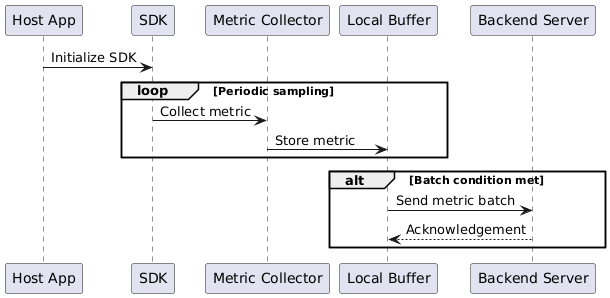
\includegraphics[width=0.8\textwidth]{figs/sequence_diagram.png}
    \caption{Sequence Diagram of SDK Data Collection and Transmission}
    \label{fig:sdk_sequence}
\end{figure}

\section{Backend Server Design}
\label{sec:backend}


The backend has four jobs: it receives metrics from the devices, authenticates users, exposes APIs for the frontend, and runs the regression detection algorithms.

When a batch of metrics arrives from the SDK, the backend validates the request, enriches each record with device cohort information, and writes the data into the time-series database.
After that, the frontend can query the stored metrics through REST endpoints, and the regression detection engine runs in the background to analyse new data as soon as it arrives.

\subsection{Database Design}

The backend uses two types of databases: a time-series database for performance metrics, and a relational database for information about users, their projects and settings.
A dedicated time-series store was chosen because it is optimized to handle large volumes of time-stamped data \cite{jensen-time-series}.

In addition, metrics are stored only for a limited period of time. Older data is removed automatically, which helps to keep only relevant data and also reduces storage costs.


\subsection{Performance Regression Detection Methods}
\label{sec:detection}

Since the system works on production data without any labelled examples, the selected detection methods must not rely on supervised training. They must also be computationally efficient, easy to interpret, and suitable for continuous execution inside the backend database.

\subsubsection{Data Partitioning and Cohorts}
Before applying any detection model, the incoming data must be grouped into meaningful subsets. Comparing high-end devices directly with low-end devices could easily produce false positives, because the natural hardware limits of a low-end device might be interpreted as a software regression. To avoid this, the data is partitioned along three dimensions: the metric type (for example, CPU usage or frame time), the application screen, and the device performance cohort (Low, Medium, or High). The detection algorithms are then executed independently on each subset.

\subsubsection{Threshold-based Methods}
Threshold-based detection relies on predefined Service Level Agreements (SLAs). A cohort is flagged as abnormal if its aggregated value exceeds a fixed upper limit defined by the developer:
\begin{equation}
    AggregatedValue > T_{\text{max}}
\end{equation}
This approach is very simple to implement and has a low computational cost. However, it requires manual configuration for each metric and each application, and the static thresholds do not adapt to natural changes in application behaviour. As a result, this method produces a high number of false positives and is not suitable for this system.

\subsubsection{Mean Shift Detection}
Mean shift detection is a statistical method that looks for regressions by comparing the mean of a current time window with the mean of a historical baseline window. A regression is reported if the current mean deviates from the baseline mean ($\mu_{\text{baseline}}$) by more than a given multiple of the baseline standard deviation:
\begin{equation}
    \mu_{\text{current}} - \mu_{\text{baseline}} > k \cdot \sigma_{\text{baseline}}
\end{equation}
This method works well for metrics that follow a normal distribution. However, mobile performance metrics are often highly skewed and contain many outliers, which can easily distort the mean value. For this reason, the method is not very reliable for metrics such as frame rendering time.

\subsubsection{Rolling Window Percentile Shift}
Percentile-based detection focuses on the overall user experience, because it evaluates the behaviour of the worst cases rather than the average behaviour~\cite{Nguyen2012}. The system collects data into two windows: a baseline window (for example, the previous 7 days) and a current window (for example, the last 24 hours). A high percentile, such as the 95th percentile ($P_{95}$), is then calculated for both windows. A regression is reported if the relative change exceeds a predefined percentage threshold:
\begin{equation}
    \frac{P_{95}(\text{current}) - P_{95}(\text{baseline})}{P_{95}(\text{baseline})} > Threshold
\end{equation}
This method is robust to non-normal and skewed distributions. It is especially effective for metrics such as frame rendering time and startup time, where the tail of the distribution represents the worst user experiences.

\subsubsection{Statistical Hypothesis Testing}
To confirm that an observed performance drop is a real regression and not just random noise, a non-parametric statistical hypothesis test can be applied. In this work, the Mann-Whitney U test~\cite{mann1947test} was considered, because it compares the distributions of two samples without assuming that the data follows a normal distribution. If the resulting $p$-value is lower than the chosen significance level ($\alpha = 0.05$), the null hypothesis is rejected and the change can be considered statistically significant. This step gives high confidence in the detected regression and helps to reduce the number of false alarms.

\subsubsection{Machine Learning and Forecasting}
More advanced methods, such as ARIMA forecasting or machine learning clustering, can also be used to model complex seasonal trends in the data. However, these methods usually require a large amount of labelled data, careful parameter tuning, and significant computational resources. Considering the dynamic and bursty nature of mobile telemetry, these approaches introduce unnecessary complexity and were not selected for this lightweight system.

\subsubsection{Selected Approach}
Taking the system requirements into account, the final approach combines the \textbf{Rolling Window Percentile Shift} method with a \textbf{Statistical Hypothesis Test}, both executed on partitioned device cohorts. This hybrid approach ignores brief spikes, adapts automatically to different hardware tiers, and provides a reliable way of detecting continuous performance degradation in production environments.

\section{Summary}

This chapter presented the methodology behind the proposed performance monitoring system. The design was driven by the requirements from the literature review, with an emphasis on low overhead, energy efficiency, and robustness across devices. The mobile SDK collects metrics on the user's device and sends them to the backend in batches; the backend stores them, exposes them through an API, and runs statistical regression detection on user cohorts. Together, these parts give developers automated insight into how their applications perform in production. The next chapter moves from design to implementation and discusses the technical challenges met during the development.
